\documentclass[a4paper]{amsart}
\usepackage{amssymb}
\usepackage{xcolor}
\usepackage{pgfplots}

\begin{document}

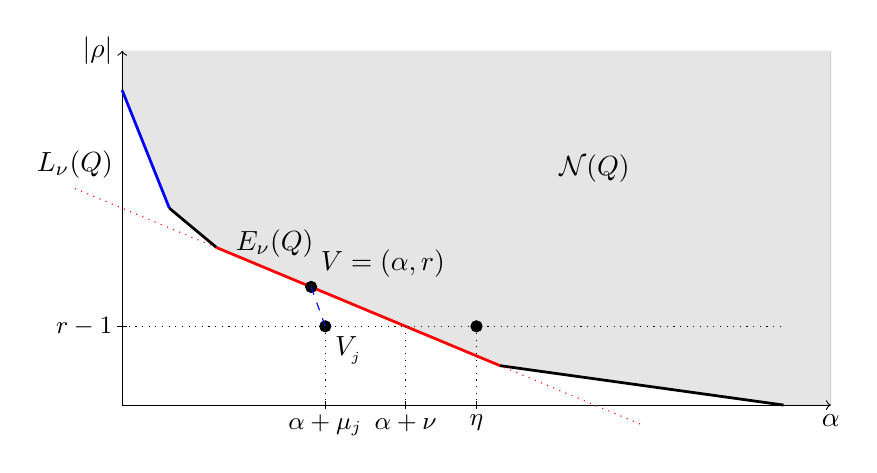
\begin{tikzpicture}[x=0.6cm,y=0.5cm]
  % fill the newton polygon
   \draw[fill=black!10, draw opacity=0.1] (0,9) -- (0,8) -- (1,5) -- (2,4) -- (8,1) --
   (14,0) -- (15,0) -- (15,9);
   \draw (10,6) node {$\mathcal{N}(Q)$};
   % axes
  \draw[->] (0,0) -- (15,0) node[anchor=north]{$\alpha$};
  \draw[->] (0,0) -- (0,9) node[anchor=east]{$|\rho|$};
  % lados
  \draw[blue,line width=1pt] (0,8) -- (1,5);
  \draw[line width=1pt] (1,5) -- (2,4);
  \draw [red,line width=1pt](2,4) -- (8,1);
  \draw [black,line width=1pt](8,1) -- (14,0);
  \draw[red,dotted] (-1,5.5) -- (11,-0.5);
  %some labels
  \draw (-1,5.5) node[anchor= south] {$L_\nu(Q)$};
  \draw (2.2, 3.5) node[anchor=south west]{$E_{\nu}(Q)$};
  \draw[fill=black] (4,3) circle[radius=2pt]
  node[anchor=south west]{$V=(\alpha,r)$};
  \draw[fill=black] (4.3,2) circle[fill=black,radius=2pt]
  node[anchor=north west]{$V_{_{j}}$};
   \draw[blue, dashed] (4,3) -- (4.3,2);
   % coordinate line r-1 and label
   \draw[dotted] (0,2) -- (14,2);
   \draw (0,2) node[anchor = east]{\small$r-1$};
   \draw (-0.1,2)--(0.1,2);
    \draw [dotted](4.3,2) -- (4.3,0); 
    \draw (4.3,0) node[anchor = north]{\small$\alpha+\mu_j$};
    \draw (4.3,0.1) -- (4.3,-0.1);%tic
  \draw [dotted](6,2) -- (6,0);
  \draw (6,0) node[anchor = north]{\small$\alpha+\nu$};
  \draw (6,0.1) -- (6,-0.1);%tic
  \draw[fill=black] (7.5,2) circle[radius=2pt];
   \draw [dotted](7.5,2) -- (7.5,0);
   \draw (7.5,0) node[anchor = north]{\small$\eta$};
   \draw (7.5,0.1) -- (7.5,-0.1);%tic

\end{tikzpicture}

\end{document}